\documentclass[12pt,a4paper]{instrumentacao}

\graphicspath{
	{../Resources/Images/}
	{../Resources/Mathematica/images/}
	{../Resources/MATLAB/images/}
}
\title{Alguns dos Efeitos Físicos Explorados em Sensores}
\author{Rogiel Sulzbach \and Rodrigo de Castro Silveira \and Yi Chen Wu}
\startdate{28 de março de 2016}
\finishdate{04 de abril de 2016}
\emails{
	\emailaddress{R.J.S.}{rogiel@rogiel.com},
	\emailaddress{R.C.S.}{csilveira.rodrigo@gmail.com} e
	\emailaddress{Y.C.}{yichenpoa@gmail.com}
}
\resume{}
\abstract{}
\keywords{}
\institute{Universidade Federal do Rio Grande do Sul, Departamento de Engenharia Elétrica, Curso de Engenharia Elétrica, Instrumentação A, Profs. Dr. Alexandre Balbinot e Dra. Léia Bagesteiro}

\headertext{Efeitos físicos}

\begin{document}
\maketitle

\todo{mudar a letra para times new roman.......}

\chapter{Introdução}
Nesta atividade de laboratório exploramos os efeitos físicos de dois tipos de sensores. Um sensor potenciométrico e outro de efeito Hall linear.

\chapter{Metodologia Experimental}
\section{Sensor potênciométrico}
Para a atividade do sensor potenciométrico, desenvolvemos um pêndulo cujo eixo estava conectado à um potenciômetro. A construção está ilustrada na figura \ref{fig:pendulo}:

\begin{figure}[H]
\centering
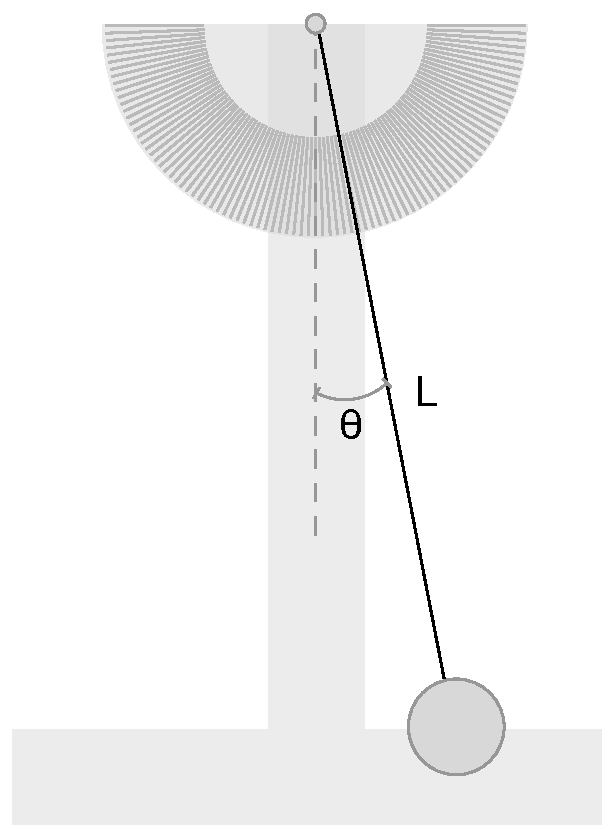
\includegraphics[width=0.4\textwidth]{Pendulo.pdf}
\caption{Estrutura do pêndulo}
\label{fig:pendulo}
\end{figure}

onde $\theta$ é o angulo de inclinação do pêndulo em relação a origem (linha tracejada).

Este pêndulo pode ser modelado eletricamente pelo seguinte circuito:

\begin{figure}[H]
\centering
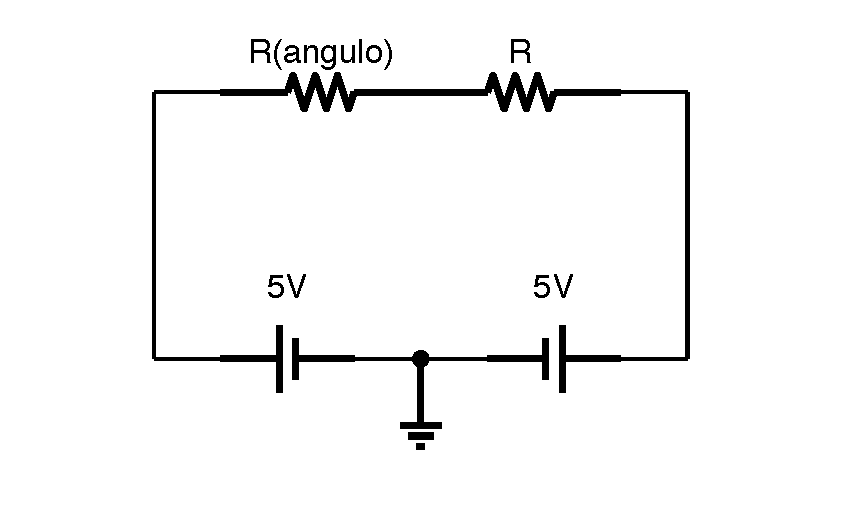
\includegraphics[width=0.6\textwidth]{Pendulo-Circuito.pdf}
\caption{Modelo elétrico do pêndulo}
\label{fig:pendulo-equivalente}
\end{figure}

onde $R(angulo)$ é uma resistência variável em função do ângulo $\theta$.

A fim de extrair a função de transferência do sensor, realiza-se um experimento com repetição onde, através de um voltímetro, mede-se a tensão elétrica sobre o resistor $R(\theta)$ em função do angulo $\theta$. Com este experimento, pode-se realizar um \textit{fit} cuja função será utilizada como a função de transferência do sensor. Uma vez que o potenciometro é linear, espera-se que a função de transferência é dada na forma da equação \ref{eq:pendulo-tf-forma} e conforme a estrutura apresentada na figura \ref{fig:pendulo}:

\begin{equation}
	R(\theta) = R_0 + R_1 \times \theta
	\label{eq:pendulo-tf-forma}
\end{equation}

onde $R(\theta)$ é a resistência elétrica em do pêndulo $\Omega$ para um dado ângulo de inclinação, $R_0$ é a resistência do pêndulo em $\Omega$ no ângulo de 0 graus, $R_1$ é a variação de resistência elétrica do pêndulo em $\Omega / rad$ em função da variação de ângulo e $\theta$ é a inclinação do pêndulo em $rad$ relativa à sua posição de repouso.

Para minimizar o efeito de \textit{ripple} de tensão elétrica da fonte de alimentação, foram utilizados 2 reguladores de tensão elétrica um \textit{LM7805}\todo{colocar o fabricante, existem vários, confirmar em cima do CI}, regulador de $(5 \pm 0.2)V$\cite{datasheet-lm7805} e um regulador \textit{LM7905}\todo{colocar o fabricante, existem vários, confirmar em cima do CI} de $(-5 \pm 0.2)V$\cite{datasheet-lm7905}. O mesmo conjunto de reguladores foi utilizado para alimentar todos componentes externos.

\subsection{Aquisição da resposta temporal do pêndulo}

Para obter a resposta temporal do pêndulo, utilizamos um mecanismo de aquisição de dados conforme a figura \ref{fig:pendulo-fluxo-medidas}:

\begin{figure}[H]
\centering
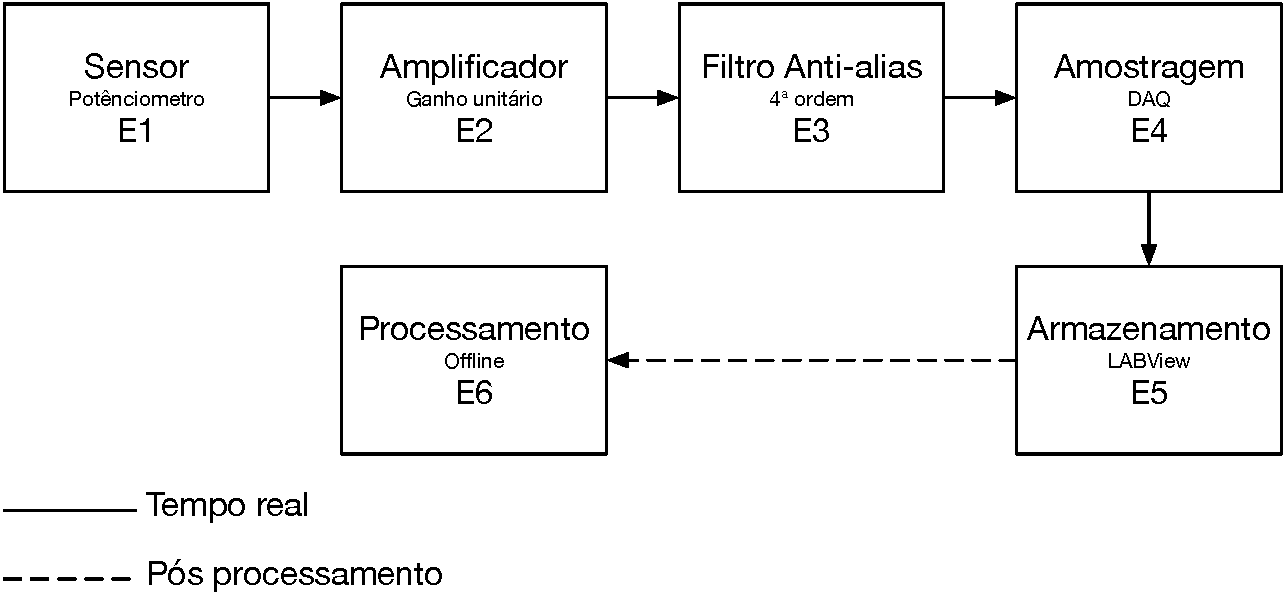
\includegraphics[width=\textwidth]{Pendulo-Fluxograma.pdf}
\caption{Fluxo de aquisição de dados do sistema.}
$E_n$ indica as etapas de aquisição de dados.
\label{fig:pendulo-fluxo-medidas}
\end{figure}

\begin{itemize}
	\item \textbf{E1}: representa o sensor utilizado, no caso deste experimento um potenciometro;
	\item \textbf{E2}: representa um amplificador com ganho unitário (buffer);
	\item \textbf{E3}: representa o filtro anti-alias utilizado para o processo de amostragem;
	\item \textbf{E4}: representa o processo de amostragem realizado utilizando o LABView e o DAQ (Data Acquisition device)
	\item \textbf{E5}: no LABView foi armazenado os dados amostrados;
	\item \textbf{E6}: após o armazenamento dos dados foi realizado o processamento destes dados.
\end{itemize}

A cadeia de medidas deste experimento pode ser representada pelo diagrama de blocos da figura \ref{fig:pendulo-cadeia-medidas}:

\begin{figure}[H]
\centering
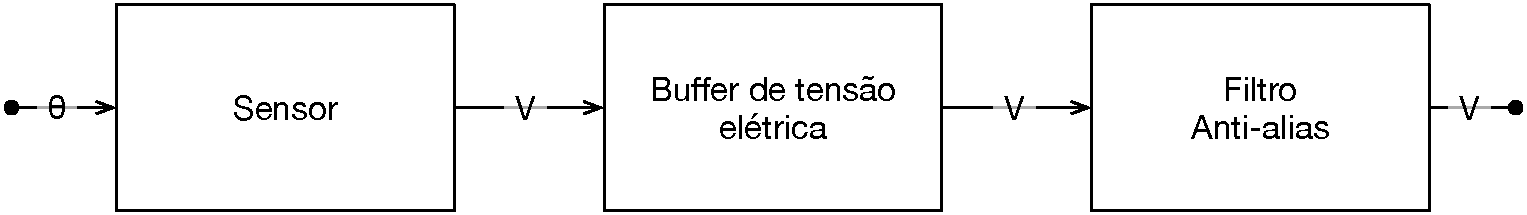
\includegraphics[width=\textwidth]{Cadeia de medida.pdf}
\caption{Cadeia de medida com grandezas de entrada e saída}
\label{fig:pendulo-cadeia-medidas}
\end{figure}

Para poder estimar o valor do angulo de inclinação do pêndulo em função da tensão elétrica medida pelo fluxo de medida mostrado na figura \ref{fig:pendulo-fluxo-medidas}, precisa-se definir a função de transferência para os 3 blocos definidos.

A função de transferência para o sensor já foi obtida no experimento anterior e é dada na equação \ref{eq:pendulo-tf-forma}. Contudo, para utilizá-la nas medidas realizadas, é preciso que a função de transferência inversa seja obtida, conforme a equação \ref{eq:pendulo-tf-forma-inversa}

\begin{equation}
	\theta = V^{-1}(\theta) = \theta_0 + \theta_1 \times V
	\label{eq:pendulo-tf-forma-inversa}
\end{equation}

onde $\theta$ é a inclinação do pêndulo em radianos, $V^{-1}(\theta)$ é a inversa da função de transferência do pêndulo modelada anteriormente, $\theta_0$ é o offset de angulo correspondente ao offset inicial de tensão elétrica e $\theta_1$ é a constante que define a variação de inclinação em função de uma variação de tensão elétrica do sensor.

A função de transferência do buffer de tensão é simples de modelar, uma vez que seu comportamento consiste em não realizar nenhuma alteração no valor de entrada, pode-se modelar usando uma função onde e saída é igual ao valor de tensão da entrada, conforme a equação \ref{eq:pendulo-tf-buffer}:

\begin{equation}
	V_{\text{buffer}} = 1 \times V_{\text{in}}	
	\label{eq:pendulo-tf-buffer}
\end{equation}

\todo{como modelar a TF do filtro?}

Por fim, pode-se calcular a função de transferência equivalente do sistema que é a concatenação de todas funções de transferência na sequência em que foram conectadas na cadeia de medida, a equação \ref{eq:pendulo-tf-concat} expressa esta relação de forma matemática:

\begin{equation}
	\theta = V_{\text{buffer}}(V_{\text{sensor}}(V_{\text{medido}}))
	\label{eq:pendulo-tf-concat}
\end{equation}

Substituindo-se estes valores, temos que a função de transferência completa do sistema é dada por \label{eq:pendulo-tf-bloco}

\begin{equation}
	\theta = V_{\text{sensor}}(V) = \theta_0 + \theta_1 \times V
	\label{eq:pendulo-tf-bloco}
\end{equation}

\chapter{Resultados e Discussões}

Com o pêndulo alimentado com a tensão elétrica simétrica de -5V e +5V, levantamos as seguintes medidas a fim de obter uma relação de tensão elétrica em função do angulo do pêndulo. A tabela \ref{tab:pendulo-calibracao} contém as medidas obtidas:

\begin{table}[H]
\centering
\caption{Tabela da relação entre temperatura e a resistência elétrica medida}
\begin{tabular}{|l|l|l|}
 \hline
 \textbf{Ângulo ($º$)} & \textbf{Tensão Elétrica ($V$)} & \textbf{Tensão Elétrica ($V$)} \\ \hline

 -60 & -1.886 & -1.886 	\\ \hline
 -55 & -1.702 & -1.702 	\\ \hline
 -50 & -1.564 & -1.564 	\\ \hline
 -45 & -1.426 & -1.426 	\\ \hline
 -40 & -1.196 & -1.196 	\\ \hline
 -35 & -1.127 & -1.127 	\\ \hline
 -30 & -0.92 & -0.92 	\\ \hline
 -25 & -0.736 & -0.736 	\\ \hline
 -20 & -0.621 & -0.621 	\\ \hline
 -15 & -0.46 & -0.46 	\\ \hline
 -10 & -0.345 & -0.345 	\\ \hline
 -5 & -0.184 & -0.184 	\\ \hline
 0 & 0. & 0. 			\\ \hline
 5 & 0.138 & 0.138 		\\ \hline
 10 & 0.322 & 0.322 	\\ \hline
 15 & 0.506 & 0.506 	\\ \hline
 20 & 0.69 & 0.69 		\\ \hline
 25 & 0.828 & 0.828 	\\ \hline
 30 & 0.966 & 0.966 	\\ \hline
 35 & 1.127 & 1.127 	\\ \hline
 40 & 1.265 & 1.265 	\\ \hline
 45 & 1.472 & 1.472 	\\ \hline
 50 & 1.587 & 1.587 	\\ \hline
 55 & 1.84 & 1.84 		\\ \hline
 60 & 1.955 & 1.955 	\\ \hline
 
\end{tabular}
\label{tab:pendulo-calibracao}
\end{table}
\todo{essa tabela ta totalmente errada. temos que refazer o experimento.} % eu fiz uma multiplicação mágica pra ajustar os valores que teríamos medido, mas precisamos mesmo fazer a medida certa dessa coisa, ou o Balbinot não vai aceitar

Observa-se que cada medida foi feita com duas repetições e de forma totalmente aleatória.

Podemos, adicionalmente, plotar estes pontos em um gráfico para melhor observar o formato da curva:

\begin{figure}[H]
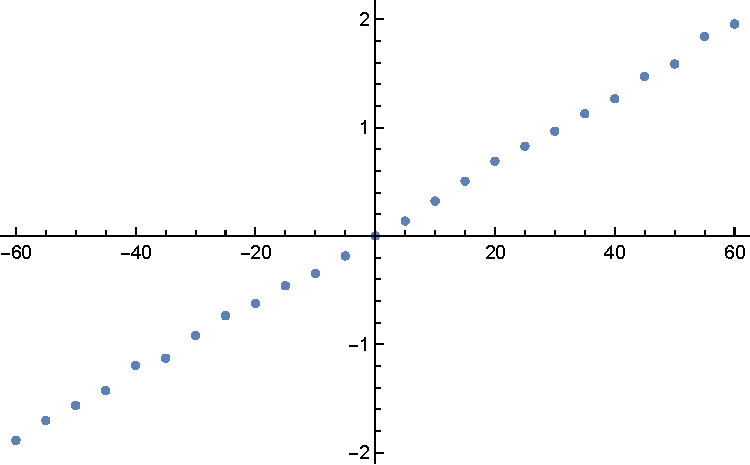
\includegraphics[width=\textwidth]{Pendulo-Pontos.pdf}
\caption{Gráfico exibindo as medidas realizadas}
\label{fig:pendulo-medidas}
\end{figure}

É fácil observar que há uma tendência linear nas medidas, então podemos realizar um ajuste de curvas a fim de tentar obter a reta que melhor representa os dados medidos. Na equação \ref{eq:pendulo-model} temos o modelo de curva que fornece o melhor ajuste:

\begin{equation}
	V(\theta) = 0.0318532 \theta +0.02116
	\label{eq:pendulo-model}
\end{equation}

onde $V(\theta)$ é a tensão elétrica do pêndulo e $\theta$ é o angulo do pêndulo em graus.

Com esta equação também é possível calcular a sua função inversa e obter o ângulo em função da tensão elétrica, na equação \ref{eq:pendulo-model-inverse}, a função inversa do modelo é dada:

\begin{equation}
	\theta(V) = -0.664297 + 31.394 V
	\label{eq:pendulo-model-inverse}
\end{equation}

Dessa forma, podemos utilizar a equação \ref{eq:pendulo-model-inverse} para calcular o angulo de um pêndulo em função de seu correspondente valor de tensão elétrica conforme será feito a seguir.

A fim de obter uma curva de tensão elétrica em função do tempo, desenvolvemos uma aplicação no LABView que fosse capaz de exibir a curva extraída em tempo real na tela e pudesse exportar estes dados de forma que pudessem ser processados externamente. Na figura \ref{fig:pendulo-labview} está mostrado uma imagem do programa utilizado.

\todo{adicionar um print do labview}

Após realizar a exportação dos dados utilizamos o software Wolfram Mathematica para importar estes dados em formato TSV (tab-separated values) e realizar o processamento. Primeiramente, precisamos notar que a informação importada está em valores de tensão elétrica (Volt) e tempo (segundo). Primeiramente, desejamos converter estes valores de tensão elétrica em uma posição angular do pêndulo e para isto, utilizamos a função inversa calculada na equação \ref{eq:pendulo-model-inverse} e a aplicamos a cada ponto medido pelo DAQ pelo LABView. \todo{precisa usar o MATLAB aqui, arrumar o texto}

A figura \ref{fig:pendulo-curva-tensao-vs-tempo} apresenta a curva em forma bruta extraída diretamente do LABView:

\begin{figure}[H]
\centering
[criar a imagem]
\caption{Curva da tensão elétrica medida no pêndulo em função do tempo}
\label{fig:pendulo-curva-tensao-vs-tempo}
\end{figure}
\todo{curva do pendulo}

Sabendo que o ângulo de oscilação do pêndulo é dado pela equação \ref{eq:pendulo-model-inverse}, é possível aplicar esta equação a cada um dos valores de tensão elétrica amostrados e converter esta curva em uma curva de posição angular em função do tempo. O resultado desta transformação está na figura \ref{fig:pendulo-curva-angulo-vs-tempo}

\begin{figure}[H]
\centering
[criar a imagem]
\caption{Curva da posição angular do pêndulo em função do tempo}
\label{fig:pendulo-curva-tensao-vs-tempo}
\end{figure}
\todo{curva do pendulo}

\begin{figure}[H]
\centering
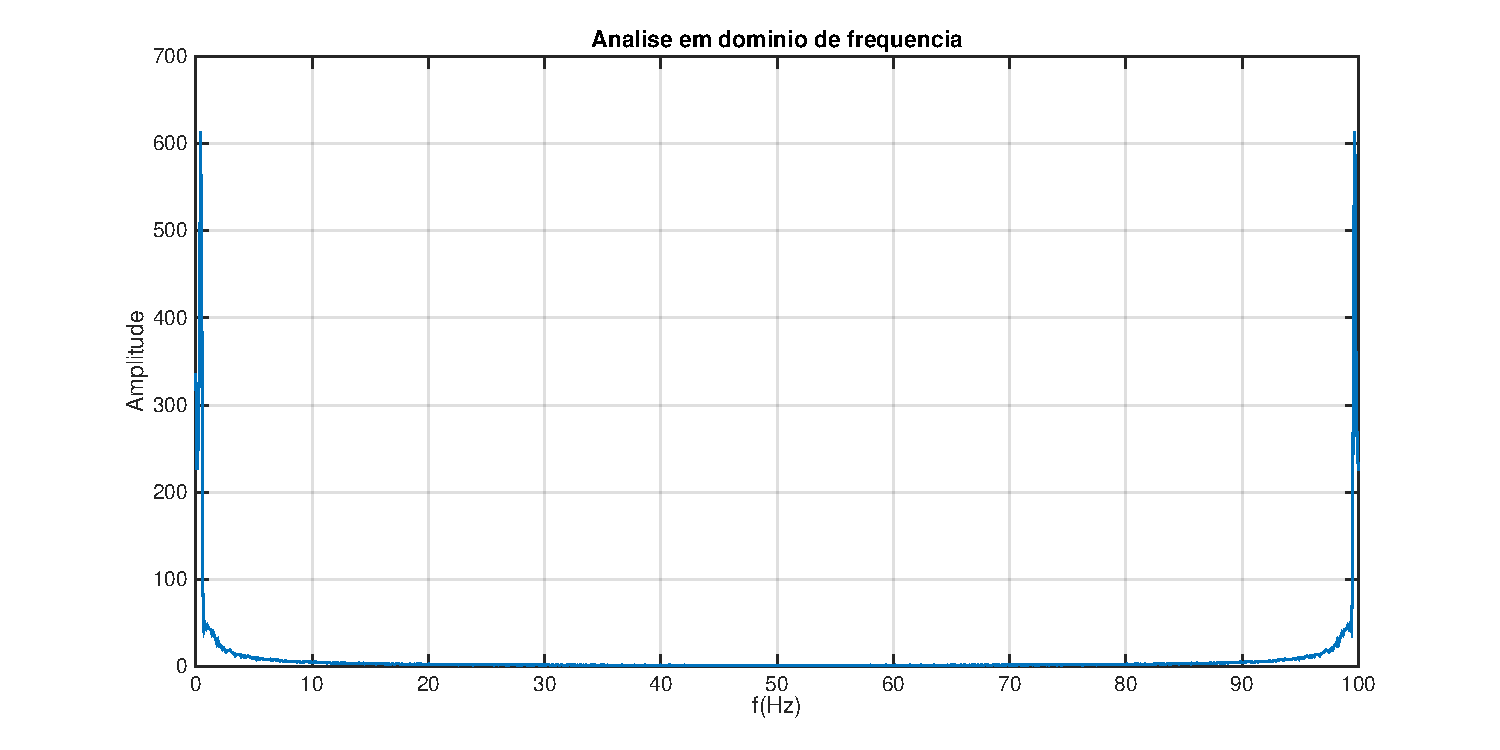
\includegraphics[width=\textwidth]{frequency-plot.pdf}
\caption{Análise de frequência da curva do pêndulo}
\label{fig:pendulo-frequencia}
\end{figure}


\section{Medição à 3 fios}

Considerando a ponte de Wheatstone da figura \ref{fig:3fios-wheatstone}

\begin{figure}[H]
\centering
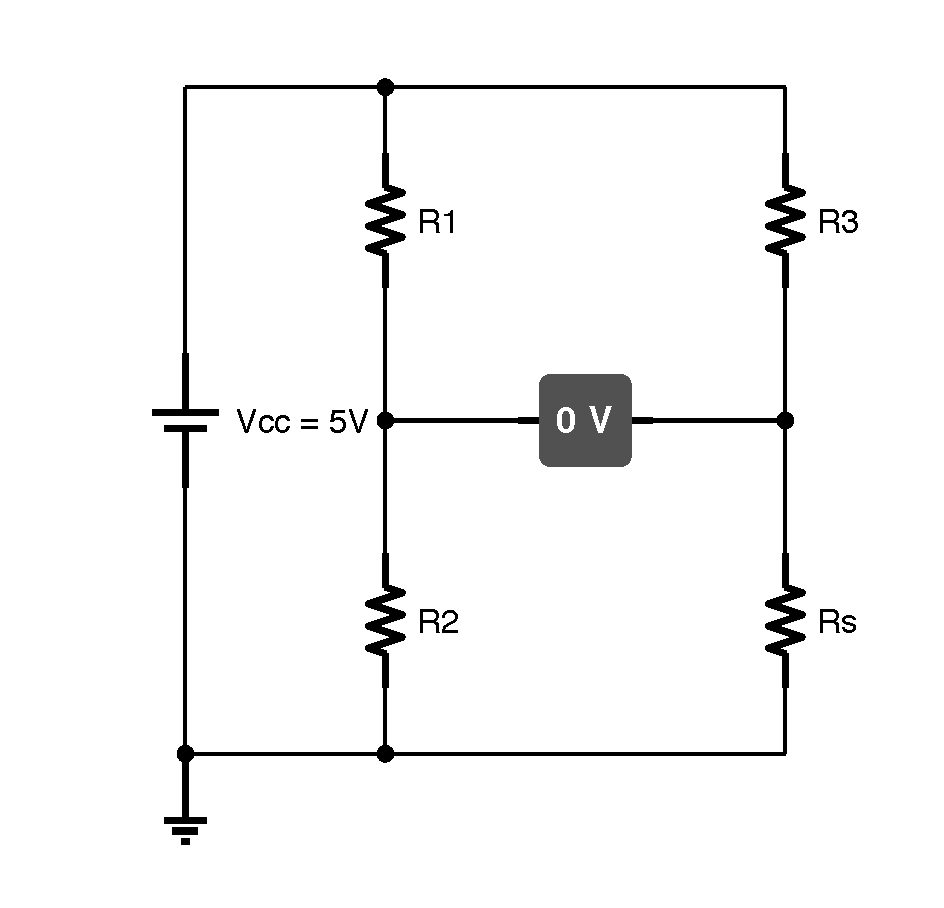
\includegraphics[width=0.6\textwidth]{Wheatstone-Bridge.pdf}
\caption{Ponte de Wheatstone equilibrada}
\label{fig:3fios-wheatstone}
\end{figure}

onde os resistores $R_1$, $R_2$ e $R_3$ são resistores fixos e definidos em função do valor de resistência máxima do sensor, $R_s$ é a resistência elétrica do sensor, variável em função da grandeza a ser medida, $V_{cc}$ é a tensão elétrica de alimentação da fonte e $V_o$ é a tensão elétrica de saída da ponte. É fácil provar que a equação correspondente ao circuito é dado pela equação \ref{eq:wheatstone-vo}:

\begin{equation}
	V_o = \left({{R_2}\over{R_1 + R_2}} - {{R_x}\over{R_x + R_3}}\right)V_{cc}
	\label{eq:wheatstone-vo}
\end{equation}

A ponte de Wheatstone pode ser visto como um circuito capaz de medir e aumentar pequenas diferenças de resistência elétrica de um sensor arbitrário em uma saída de tensão com sensibilidade maior que a sensibilidade do sensor. Isto é, para uma pequena variação, é possível obter (com uma ponte devidamente projetada) uma saída em tensão elétrica com maior sensibilidade quando comparada ao sensor isolado.

Embora esta característica seja ideal para utilizar em sensores cuja amplitude de variação de resistência elétrica seja muito pequena, isto também significa que não é possível desprezar as resistências elétricas intrínsecas dos fios de conexão do sensor com a ponte. Como a ponte de Wheatstone pode ser utilizada como um condicionador para pequenas variações de resistência elétrica, uma pequena inserção de resistência elétrica do fio pode causar um \textit{bias} significante na saída da ponte.

Com a finalidade de compensar esta não idealidade, é possível realizar medidas utilizando técnicas denominadas de \textbf{medida à 3 fios} e \textbf{medida à 4 fios}.

Nestas técnicas, um fio com as mesmas especificações de comprimento, seção reta e material é utilizado com a finalidade de tentar obter uma resistência elétrica semelhante ao fio de conexão do sensor e minimizar a significância do fio na medida. Este método pode ser expresso pelo seguinte circuito elétrico equivalente da figura \ref{fig:wheatstone-wire-model}:

\begin{figure}[H]
\centering
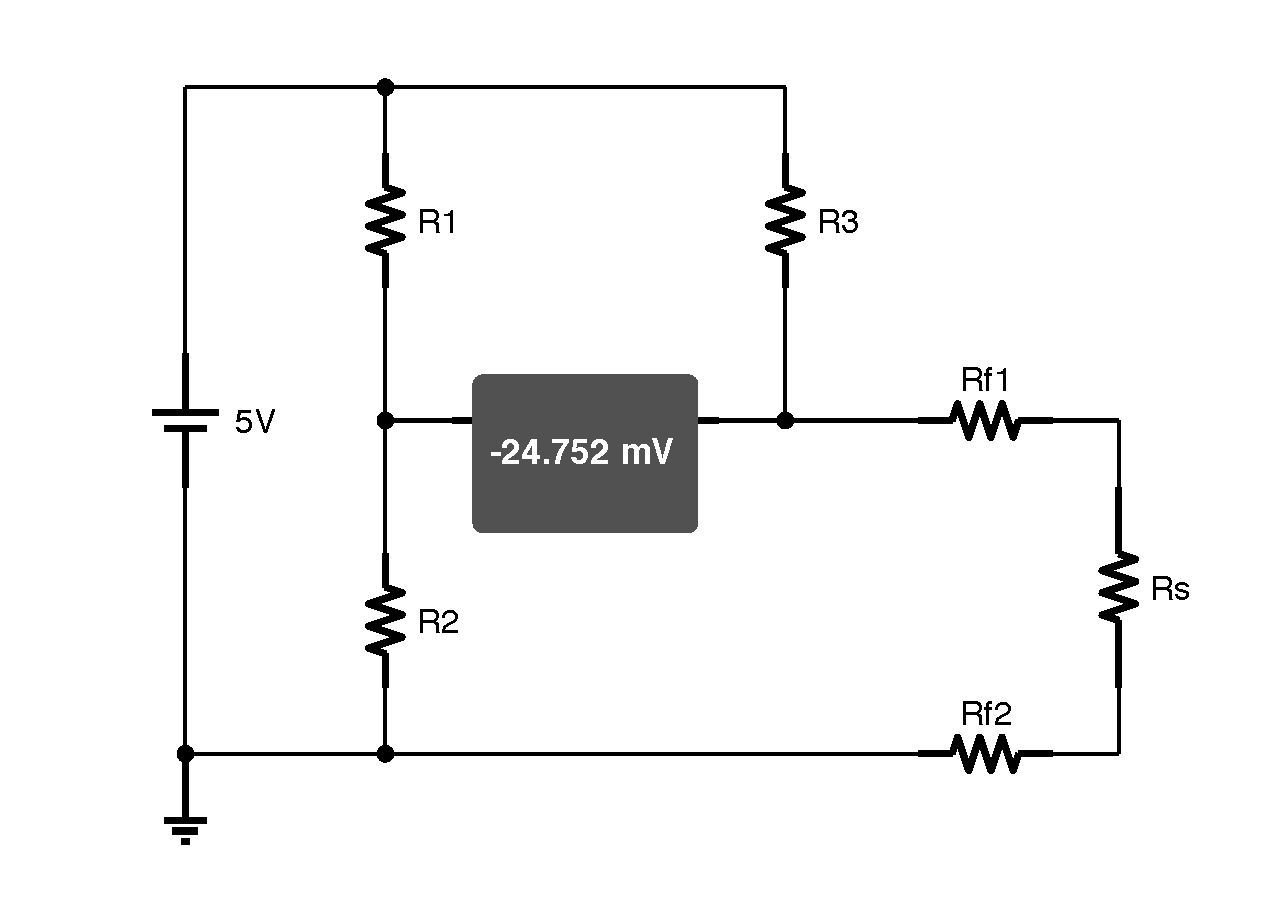
\includegraphics[width=0.6\textwidth]{Wheatstone-Bridge-WiresModel.pdf}
\caption{Ponte de Wheatstone com a resistência elétrica dos fios}
\label{fig:wheatstone-wire-model}
\end{figure}

onde os resistores $R_1$, $R_2$ e $R_3$ são resistores fixos e definidos em função do valor de resistência máxima do sensor, $R_s$ é a resistência elétrica do sensor, variável em função da grandeza a ser medida, $V_{cc}$ é a tensão elétrica de alimentação da fonte e o resistores $R_f$ são resistências intrínsecas dos fios e espera-se que para fios de mesmo material, comprimento e seção reta, seus valores sejam semelhantes.

Conforme observa-se na figura \ref{fig:wheatstone-wire-model}, para os mesmos valores de $R_1$, $R_2$, $R_3$ e $R_f$ o valor de tensão elétrica de saída da ponte é diferente de zero. Isto é causado devido ao desbalanceamento da ponte causado pela resistência elétrica dos fios de conexão do sensor, representados por $R_{f1}$ e $R_{f2}$. Caso o sensor tenha uma variação pequena de resistência elétrica, o \textit{bias} causado pelas resistências série pode ser muito significante e gerar um erro absurdo. Para reduzir o impacto dessa resistência série, pode-se utilizar o método de medida à 3 fios, onde um terceiro fio é conectado diretamente entre o sensor e um dos terminais do voltímetro, conforme figura \ref{fig:wheatstone-3wire}.

\begin{figure}[H]
\centering
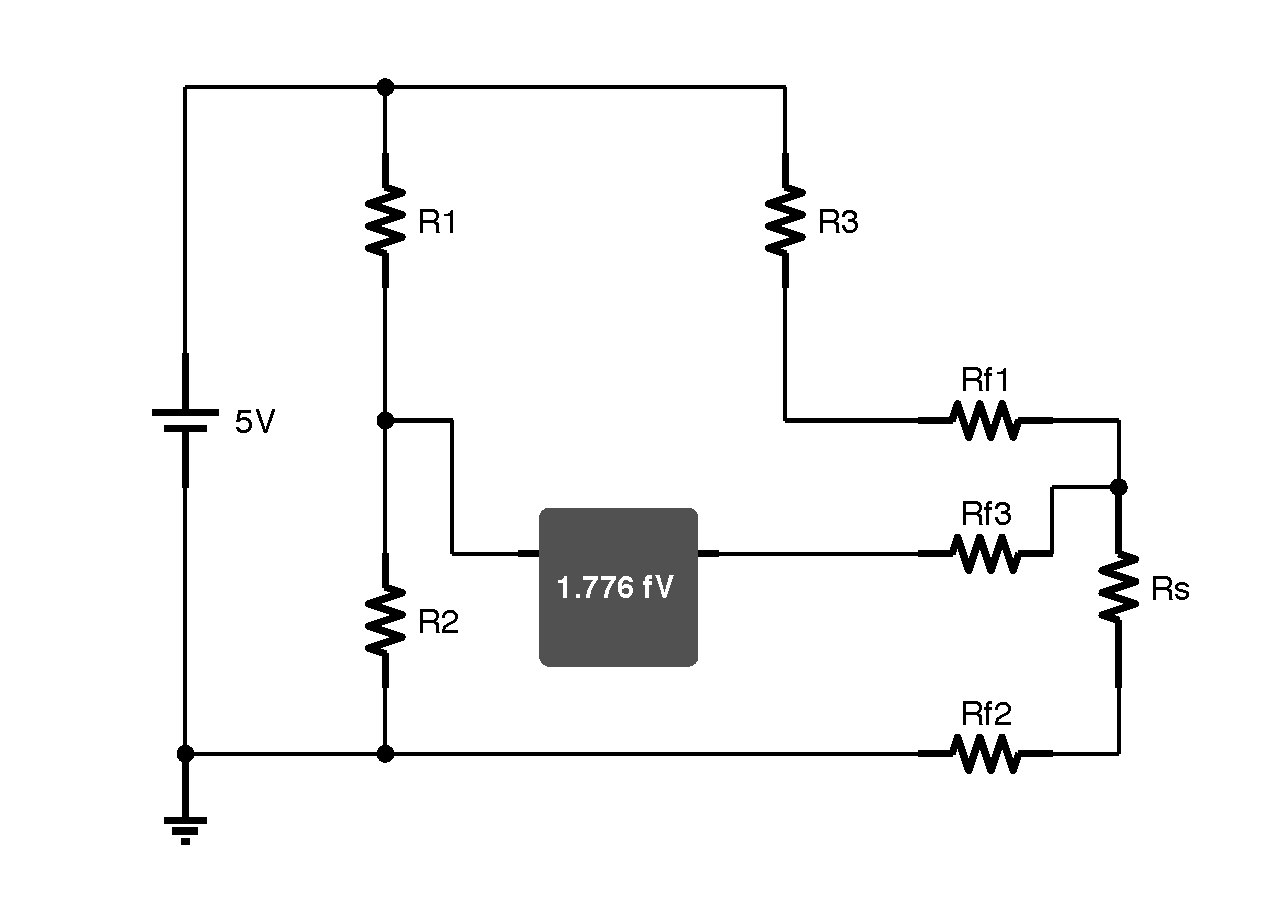
\includegraphics[width=0.6\textwidth]{Wheatstone-Bridge-3Wire.pdf}
\caption{Ponte de Wheatstone com medida à 3 fios}
\label{fig:wheatstone-3wire}
\end{figure}

onde foi adicionado um terceiro fio representado pela resistência $R_{f3}$ que representa a resistência elétrica do fio de conexão direta entre o voltímetro e o sensor. Nota-se que para que o método seja eficaz, é necessário que o voltímetro tenha uma impedância elétrica muito alta a fim de evitar que haja uma queda de tensão elétrica sobre o resistor $R_{f3}$.

É possível observar claramente no resultado da simulação que o \textit{bias} produzido por esta construção ficou em $1.776 fV$, que dada a sensibilidade de um multímetro comercial de baixo custo, é imperceptível e a incerteza é no mínimo 1000x superior (na ordem de mV).

\todo{equacionar isso}

\section{Medição à 4 fios}

Embora o método à 3 fios melhore bastante a qualidade da medida, há um offset dependente de $R_{f2}$ que considerando o comprimento do fio pode ser significante e afetar o resultado para sensores com baixas resistências elétricas associado com pequenas variações. Para solucionar este problema, há um outro método de medida que utiliza 4 fios e 2 instrumentos para realizar a medida com maior precisão, este método é denominado de \textbf{método à 4 fios}. Nele, é associado um amperímetro em série com o sensor e um voltímetro em paralelo com o mesmo e através de lei de Ohm, pode-se extrair o valor de resistência do sensor. Na figura \ref{fig:4wire-circuit} está apresentado o esquemático elético equivalente deste método.

\begin{figure}[H]
\centering
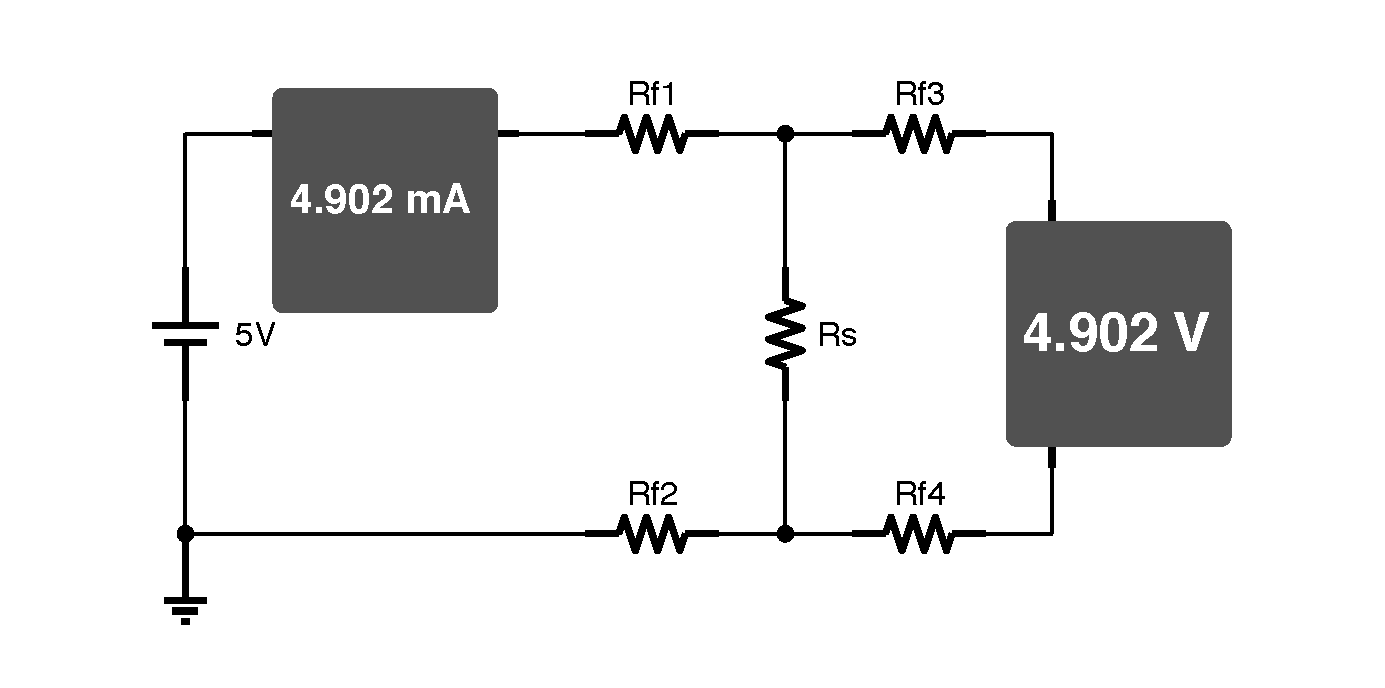
\includegraphics[width=0.6\textwidth]{4WireMeasure.pdf}
\caption{Esquemático elétrico do método de medida à 4 fios}
\label{fig:4wire-circuit}
\end{figure}

onde $R_s$ é a resistência elétrica do sensor e $R_f$ são as resistências elétricas dos fios de conexão do sensor e dos instrumentos.

Neste método, aplica-se diretamente a lei de Ohm conforme a equação \ref{eq:ohm}:

\begin{equation}
	R_s = \frac{V_s}{I_s}
	\label{eq:ohm}
\end{equation}

Independente da resistência elétrica dos fios, considerando que a impedância do voltímetro seja infinita ou muito grande, a queda de tensão provocada por $R_{f3}$ e $R_{f4}$ são negligenciáveis e a tensão medida sobre $R_s$ é a tensão real (respeitando a incerteza do instrumento). Para as resistências $R_{f1}$ e $R_{f2}$ a corrente elétrica que circula por elas é a mesma que circula por $R_s$, embora elas provoquem uma redução da corrente elétrica que circula pelo ramo, este é compensado na redução de tensão medida $V_s$. Logo, considerando-se somente o erro devido as conexões, o erro causado por esta construção é zero ou negligenciável.

\todo{medida a 3 fios - só calcular}

%%%%%%%%%%%%%%%%%%%%%%%%%%%%%%%%%%%%%%%%%%%%%%%%%%%%%%%%%%%%%%%%%%%%%%%%%%%%%%

\todo{sensibilidade, resolução de entrada, resolução de saída, erro de linearidade ou de conformidade, incerteza, etc, assim como, a correspondente Cadeia de Medidas Proposta (teórica) e a Cadeia de Medidas Experimental}

\todo{labview+matlab}
\todo{só matlab}

\todo{determinar a sensibilidade, a resolução de entrada, resolução de saída, o erro de linearidade (ou erro de conformidade se for o caso) de seu sistema}

\todo{Tarefa para Casa: de posse da função de medição de seu sistema determinar a incerteza combinada deste sistema.}

\todo{com os sinais armazenados pelo programa LabVIEW elaborar um procedimento para determinar o decaimento em função do tempo e discutir esse resultado.}

\todo{Medição da Amplitude.}
\todo{Medição de $\theta_0$}
\todo{incertezas dos itens anteriores e dos comprimentos}

\todo{amortecimento}

\todo{medição do periodo}
\todo{grafico de amplitude e periodo}

\todo{modelo de thevenin}
\todo{grafico saida do pot vs angulo. qual erro?}
\todo{sensibilidade do circuito anterior}

\todo{discutir quantidade de amostras (medidas obtidas) para cada ângulo versus tensão.}
\todo{calcular a incerteza de TODAS medidas}


\todo{experimento do efeito hall}
\todo{experimento do led}

\chapter{Conclusões}

\chapter*{Anexos}
\section{Mathematica}
%\includenotebook{../Resources/Mathematica/Experimento 1-1.pdf}{Experimento 1}

\section{LabVIEW}

\section{MATLAB}

\begin{thebibliography}{9}
\bibitem{mathematica-numerial-precision} \url{https://reference.wolfram.com/language/tutorial/NumericalPrecision.html}, acessado em 16 de março de 2016

%\bibitem{ref1} Sobrenome, A.B.; Sobrenome, C.D. Title of the cited article. Journal Title 2007, 6, 100-110. 
%\bibitem{ref2} Balbinot, A.; Brusamarello, V.J.. Title of the cited article. Journal Title 2007, 6, 100-110. 
%\bibitem{ref3} Author, A.; Author, B. Title of the chapter. In Book Title, 2nd ed.; Editor, A., Editor, B., Eds.; Publisher: Publisher Location, Country, 2007; Volume 3, pp. 154-196.
%\bibitem{ref4} Author, A.; Author, B. Book Title, 3rd ed.; Publisher: Publisher Location, Country, 2008; 
%pp. 154-196.

\todo{formatar essas referencias da forma correta... nao sei como ele quer}
\bibitem{datasheet-lm7805} Datasheet oferecido pelo fabricante do regulador de tensão LM7805
\bibitem{datasheet-lm7905} Datasheet oferecido pelo fabricante do regulador de tensão LM7905

\todo{arrumar bibliografia}

\end{thebibliography}

\end{document}
